\notechapter{N-20240608}{Plane Curves: Equations, Singularities, and Projective Closure}

\section{Curves as equations}

A plane algebraic curve is the zero set of a polynomial:
\[
  C=V(f)=\{(x,y)\in k^2:f(x,y)=0\}.
\]
This simple definition changes the meaning of geometry. A curve is no longer just a drawn shape; it is controlled by an algebraic equation.

\[
\begin{array}{c|c}
f(x,y) & \text{curve}\\
\hline
y-mx-b & \text{line}\\
x^2+y^2-1 & \text{circle}\\
y^2-x^3 & \text{cusp}\\
y^2-x^2(x+1) & \text{nodal cubic}
\end{array}
\]

\begin{figure}[H]
\centering
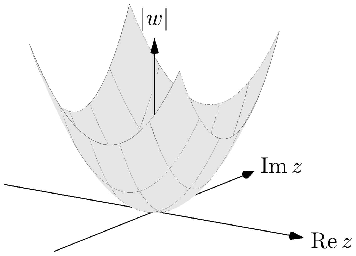
\includegraphics[width=.55\linewidth]{figures/N-20240608/parabola.pdf}
\caption{A familiar curve can be treated as an equation, not only as a picture.}
\end{figure}

\section{Coordinate rings}

The coordinate ring of \(C=V(f)\) is
\[
  k[C]=k[x,y]/(f).
\]
Two polynomials define the same function on the curve if they differ by a multiple of \(f\). So \(k[C]\) is the algebra of polynomial functions living on the curve.

This is one of the main ideas of algebraic geometry:
\[
  \text{study a space by studying its functions.}
\]

\section{Irreducibility}

If \(f=gh\), then
\[
  V(f)=V(g)\cup V(h).
\]
So factorization of polynomials corresponds to decomposition of curves.

For example, \(xy=0\) is the union of the two coordinate axes. It is reducible. A curve given by an irreducible polynomial is a single algebraic piece.

\section{Singular points}

A point \(p=(a,b)\in C\) is singular if
\[
  f(a,b)=0,\qquad f_x(a,b)=0,\qquad f_y(a,b)=0.
\]
At such a point, the usual tangent line is not well-defined by the linear approximation because the linear part vanishes.

For the cusp \(y^2=x^3\), the origin is singular. For the node \(y^2=x^2(x+1)\), the origin is also singular, but the local shape is different. A cusp has one branch with a sharp turn; a node has two branches crossing.

\section{Tangent cones}

If the lowest-degree nonzero part of \(f\) at a point is \(f_d\), then \(f_d=0\) describes the tangent cone. For a smooth point, this is just one tangent line. For a node, it can be two lines.

Example:
\[
  f(x,y)=y^2-x^2-x^3.
\]
The lowest-degree part is
\[
  y^2-x^2=(y-x)(y+x),
\]
so the tangent cone at the origin consists of the two lines \(y=x\) and \(y=-x\).

\section{Projective closure}

Affine curves can hide points at infinity. To see the whole curve, homogenize the equation. If
\[
  f(x,y)=y-x^2,
\]
then the homogenized equation is
\[
  F(x,y,z)=yz-x^2.
\]
The projective closure is \(V(F)\subset\mathbb P^2\). In the chart \(z=1\), we recover the original parabola. On the line at infinity \(z=0\), we get \(-x^2=0\), so \(x=0\), giving the point \([0:1:0]\).

Projective closure is the operation of filling in the missing directions at infinity.

\section{Bezout as a guiding principle}

A first form of Bezout's theorem says that two projective plane curves of degrees \(m\) and \(n\) meet in \(mn\) points, counted with multiplicity, over an algebraically closed field, provided they have no common component.

Its meaning is that projective geometry restores the correct accounting. Missing intersections at infinity and tangencies are not exceptions; they are counted correctly once the setting is projective and multiplicities are included.

%% expanded-on-review

\section{A coordinate-ring computation}

For the cusp
\[
  C=V(y^2-x^3),
\]
the coordinate ring is
\[
  k[C]=k[x,y]/(y^2-x^3).
\]
A useful parametrization is
\[
  x=t^2,\qquad y=t^3.
\]
This gives a map
\[
  k[x,y]/(y^2-x^3)\longrightarrow k[t],
  \qquad x\mapsto t^2,\quad y\mapsto t^3.
\]
The image is \(k[t^2,t^3]\), not all of \(k[t]\). This algebraic fact remembers the cusp: near the origin the curve is not as smooth as a line.

For the parabola \(y=x^2\), by contrast, the coordinate ring is just \(k[x]\). Algebraically it behaves like a line. This comparison is a good way to feel what singularities do: they make the function ring less simple.

\section{Intersection multiplicity by example}

Consider the line \(y=0\) and the parabola \(y=x^2\). They meet at the origin. Substituting \(y=0\) into \(y=x^2\) gives
\[
  x^2=0.
\]
So the intersection has multiplicity \(2\). Geometrically, the line is tangent to the parabola.

This small example explains why Bezout counts multiplicity. If one only counts visible points, a tangent intersection looks like one point. Algebra sees that the contact is doubled.

\section{Why projective closure changes counting}

The affine lines \(y=0\) and \(y=1\) do not meet in \(\mathbb A^2\). After homogenizing, they become
\[
  y=0,\qquad y-z=0.
\]
In \(\mathbb P^2\), they meet at \([1:0:0]\). Thus projective closure does not add decorative points; it repairs the accounting of intersections.

This is the same philosophy as projective geometry in the previous note, now applied to polynomial curves.


\section{What to remember}

Plane curves sit at the meeting point of algebra and geometry:
\[
\begin{array}{c|c}
\text{geometry} & \text{algebra}\\
\hline
\text{curve} & \text{polynomial equation}\\
\text{functions on the curve} & \text{coordinate ring}\\
\text{decomposition} & \text{factorization}\\
\text{singular point} & f=f_x=f_y=0\\
\text{points at infinity} & \text{homogenization}
\end{array}
\]
